\subsection{Mathematical Primer: Basic Models}

A coverage of the essentials of mathematics behind quantitative trading. May overlap the earlier section on mathematical primer.

\subsubsection{Univariate Time Series Models}

Trading activities through an exchange can be described by a sequence of time stamps ('ticks') $t_0 < t_1 < \cdots < t_n$, and 'marks' $y_i$ at time $t_i$, where $t_i$ denote market open, $t_n$ denote market close. The marks $y_i$ is a characteristic of the order book at time of $i$th activity. Events with marks associated with the ticks can be described mathematically as a marked point process.
\begin{figure}[H]
\centering
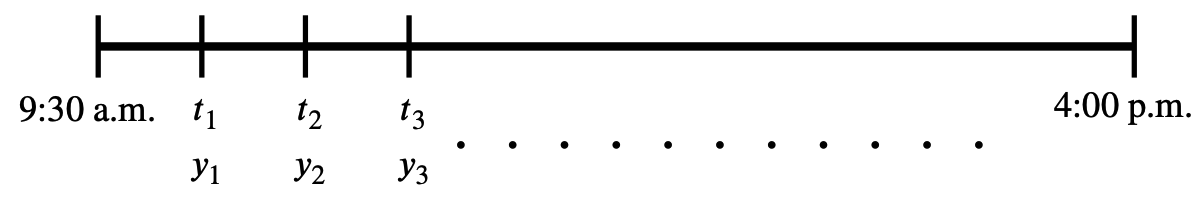
\includegraphics[scale=0.4]{/fundamentals/ticksandmarks}
\caption{Ticks and Marks}
\end{figure}

A data aggregation method is where aggregation is conducted when there is a change in marker. An alternative aggregation method would be to divide the time span $T$ for exchange hours into $K$ intervals, so regularly spaced intervals are of size $\Delta t = T/K$. The time series method to be discussed will apply to all aggregated data.\\

Let $p_{it} = \ln P_{it}$ denote price of $i$th asset at time $t$; $p_t = (p_{1t}, p_{2t}, \ldots, p_{nt})$ denote price vector for $n$ assets; $y_{it}$ denote vector of characteristics of $i$th asset at time $t$. These quantities are aggregated from high frequency data. Consider $r$ factors $f_t = (f_{1t}, f_{2t}, \ldots, f_{rt})$ that may include market and industry factors, and asset characteristics. Trading rules can be broadly grouped as follows:
\begin{enumerate}[label=\roman*.]
\setlength{\itemsep}{0pt}
\item \hlt{Statistical Arbitrage}: $E(p_{i, t+1} \ \vert \ p_{i,t}, p_{i, t-1}, \ldots, y_{i,t}, y_{i, t-1}, \ldots)$, that predicts the price of $i$th stock at $t+1$ based on past trading information (also known as time series momentum)
\item \hlt{Momentum}: $E(p_{t+1} \ \vert \ p_t, p_{t-1}, \ldots, y_t, y_{t-1}, \ldots)$, that predicts the cross-sectional momentum of a subset of stocks based on past trading characteristics. For portfolio formation and rebalancing, pairs trading
\item \hlt{Fair Value}: $E(p_{t+1} \ \vert \ p_{t}, p_{t-1}, \ldots, y_t, y_{t-1}, \ldots, f_t, f_{t-1}, \ldots)$, predicts price using all relevant quantities. Factors normally include market, Fama-French; at a more macro level than timescale considered for price prediction, but may still be useful.
\end{enumerate}

Hence price and volatility prediction can be formulated as a time series prediction problem. Autocorrelations and partial autocorrelations can be used to build autoregressive and ARCH models with some predictive power.\\

Let $Y_1, Y_2, \ldots, Y_T$ be a sequence of random variables with a joint probability distribution. A sequence of observations of stochastic process $\{Y_t, t = 1, \ldots, T\}$ is a realisation of the process.\\
A time series $\{Y_t\}$ is \hlt{stationary} if for every integer $m$, the set of variables $Y_{t_1}, Y_{t_2}, \ldots, Y_{t_m}$ depends only on the distance between times $t_1, t_2, \ldots, t_m$. Thus $E(Y_t) = \mu$, $Var(Y_t) = \sigma^2$ are constant for all $t$.\\
The \hlt{auto-covariance} function is defined as
\begin{equation}
\gamma(s) = Cov(Y_t, Y_{t-s}) = E[(Y_t - \mu)(Y_{t-s} - \mu)] \ \ \forall s = 0, \pm 1, \ldots \nonumber
\end{equation}
The \hlt{auto-correlation} of process at lag $s$ is defined as
\begin{equation}
\rho(s) = Corr(Y_t, Y_{t-s}) = \frac{Cov(Y_t, Y_{t-s})}{\left(Var(Y_t) \ Var(Y_{t-s}) \right)^{1/2}} = \frac{\gamma(s)}{\gamma(0)}, \ \ \ \forall s = 0, \pm 1, \ldots \nonumber
\end{equation}

Some examples of stationary stochastic processes are as follows:

\begin{example} \hlt{(White Noise)} Sequence of discrete independent random variables (r.v.) $\{\epsilon_t \}$ with $E[\epsilon_t] = 0$ and $E[\epsilon_t^2] = \sigma^2$. Set $Y_t = \mu + \epsilon_t$, then $E[Y_t] = \mu$, $Cov(Y_t, Y_{t-s}) = Var(Y_t) = \sigma^2$ if $s=0$, and $Cov(Y_t, Y_{t-s}) = 0$ if $s \neq 0$. Hence the process is stationary.
\end{example}

\begin{example} \hlt{(Moving Average)} Let $\{\epsilon_t\}$ be independent r.v., with process $\{Y_t\}$ where $Y_t = \mu + \epsilon_t + \epsilon_{t_1}$ for $t = 0, 1, 2, \ldots$, and $\mu$ is constant. Then $E[Y_t] = \mu \ \forall t$, and
\begin{equation}
Cov(Y_t, Y_{t-s}) = \gamma(s) = 
\begin{cases}
2 \sigma^2 \ \ \text{if } s = 0 \\
\sigma^2 \ \ \text{if } s = 1 \\
0 \ \ \text{if } s > 1
\end{cases} \nonumber
\end{equation}
Hence $\{Y_t\}$ is stationary, with $\rho(s) = \gamma(s) / \gamma(0)$ such that $\rho(0) = 1$, $\rho(1) = 1/2$, $\rho(s) = 0$ for $\abs{s} > 1$.
\end{example}

Some examples of non-stationary stochastic processes are as follows:

\begin{example} \hlt{(Random Walk with Drift)} Let $\{\epsilon_t \}$ be sequence of independent r.v. with  $E[\epsilon_t] = 0$, $E[\epsilon_t^2] = \sigma^2$, and define process $\{Y_t\}$ by $Y_t = Y_{t-1} + \delta + \epsilon_t$ with $Y_0 = 0$. Then the process can be summarised as
\begin{equation}
Y_t = \delta t + \sum\limits_{j=1}^t \epsilon_j \nonumber
\end{equation}
Note that $E[Y_t] = \delta t$ and $Var[Y_t] = t \sigma^2$, hence process $\{Y_t\}$ is not stationary.
\end{example}

Given $T$ observations from stationary process $\{Y_t\}$, the \hlt{sample mean} is $\overline{Y} = \frac{1}{T} \sum\limits_{t=1}^T Y_t$. The \hlt{sample auto-covariance} function is defined by $\hat{\gamma}(s) = \frac{1}{T} \sum\limits_{t=1}^{T-s} (Y_t - \overline{Y})(Y_{T-s} - \overline{Y})$ for $s=0, 1, \ldots$. The \hlt{sample auto-correlation} function (ACF) is defined as $\hat{\rho}(s) = \frac{\hat{\gamma}(s)}{\hat{\gamma}(0)} = r(s)$. The \hlt{sample variance} is $Var(\overline{Y}) = \frac{\gamma(0)}{T}\left[1 + 2 \sum\limits_{u=1}^{Y-1} \left(\frac{T-u}{T} \right) \rho(u) \right]$; note that it has to account for auto-correlations.

\begin{definition} A stochastic process $\{Y_t\}$ is a \hlt{linear process} if it can be represented as
\begin{equation}
Y_t = \mu + \sum\limits_{j=0}^{\infty} \Psi_j \epsilon_{t-j} \nonumber
\end{equation}
where $\epsilon_t$ are independent with mean $0$, variance $\sigma_{\epsilon}^2$, and $\sum\limits_{j=0}^{\infty} < \infty$.
\end{definition}


